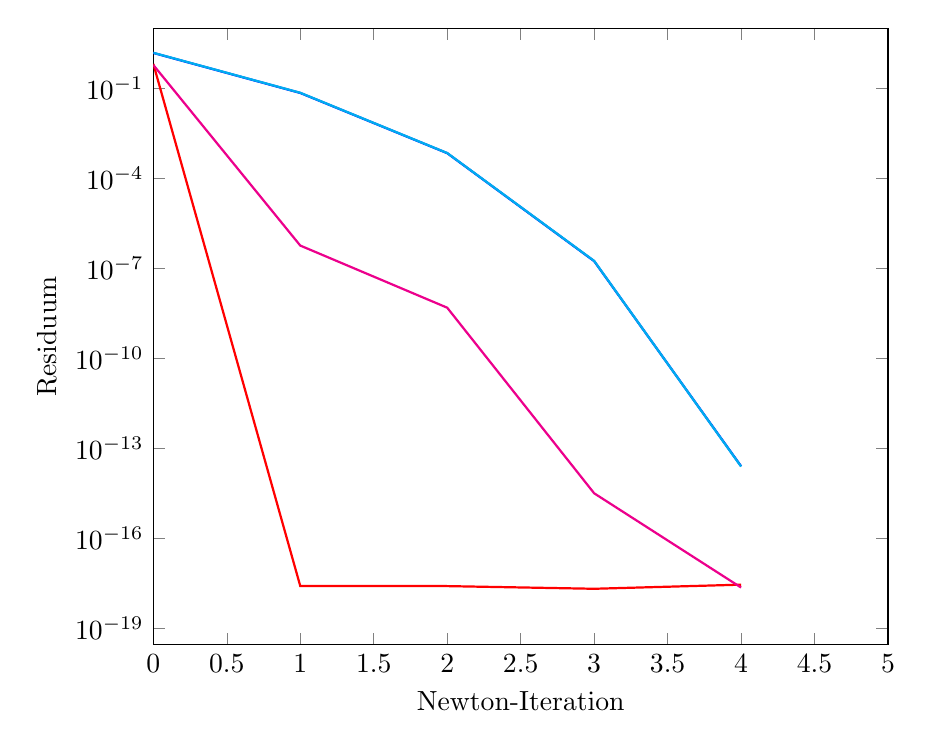
\begin{tikzpicture}[every plot/.append style={thick}] 
\begin{axis}[ 
label style={font=\normalsize}, 
xlabel={Newton-Iteration}, 
ylabel={Residuum}, 
xmin=0, xmax=5, 
ymode=log, 
ymin=0, ymax=10, 
width=0.9\textwidth, 
grid style=dashed, 
] 
\addplot[ 
color=blue, 
] 
coordinates { 
(0, 1.50e+00)(1, 6.94e-02)(2, 6.81e-04)(3, 1.71e-07)(4, 2.47e-14)}; 
\addplot[ 
color=red, 
] 
coordinates { 
(0, 6.50e-01)(1, 2.50e-18)(2, 2.48e-18)(3, 2.02e-18)(4, 2.77e-18)}; 
\addplot[ 
color=cyan, 
] 
coordinates { 
(0, 1.52e+00)(1, 7.04e-02)(2, 6.89e-04)(3, 1.74e-07)(4, 2.41e-14)}; 
\addplot[ 
color=magenta, 
] 
coordinates { 
(0, 5.96e-01)(1, 5.65e-07)(2, 4.78e-09)(3, 3.09e-15)(4, 2.22e-18)}; 
\end{axis} 
\end{tikzpicture} 
